\chapter{Implementasi dan Pengujian}
\label{chap:implementasi&pengujian}

Pada bab ini akan dijelaskan mengenai implementasi perangkat lunak, serta pengujian perangkat lunak. Implementasi perangkat lunak berisi penjelasan lingkungan pengembangan perangkat lunak dan hasil implementasi. Sedangkan pengujian perangkat lunak berisi hasil pengujian fungsional dan eksperimental terhadap perangkat lunak yang telah dibangun.

\section{Implementasi}

\subsection{Lingkungan Implementasi}
\label{lingkungan_implementasi}
Implementasi perangkat lunak ini dilakukan di komputer penulis dengan spesifikasi berikut:
\begin{enumerate}
    \item \textit{Processor}: Intel Core i5-10300H
    \item \textit{Random Access Memory(RAM)}: 16 GB DDR4
    \item Sistem Operasi: Windows 10
    \item Versi Java: 1.8.0\_291
    \item Versi JavaFX: 8.0.202
    \item Versi Netbeans: 12.1
    \item Versi Scenebuilder: 11.0.0
\end{enumerate}

\subsection{Hasil Implementasi}
Implementasi berupa aplikasi \textit{screensaver}, dimana aplikasi tersebut akan dijalankan secara otomatis setelah komputer tidak digunakan selama beberapa saat. Gambar \ref{fig:5_hasil} dan \ref{fig:5_hasil2} merupakan tampilan dari aplikasi \textit{screensaver}. Dikarenakan pada Portal Akademik Mahasiswa tidak terdapat foto mahasiswa, maka foto digantikan dengan \textit{base64 image} yang dimasukkan secara \textit{hardcode}. \textit{Layout} dari aplikasi disimpan dalam \textit{file} bertipe FXML (lampiran ...). \textit{file} FXML tersebut tidak dibuat secara manual, melainkan dengan menggunakan aplikasi Scene Builder\footnote{\url{https://gluonhq.com/products/scene-builder/}}. 

\begin{figure}[H]
	\centering
	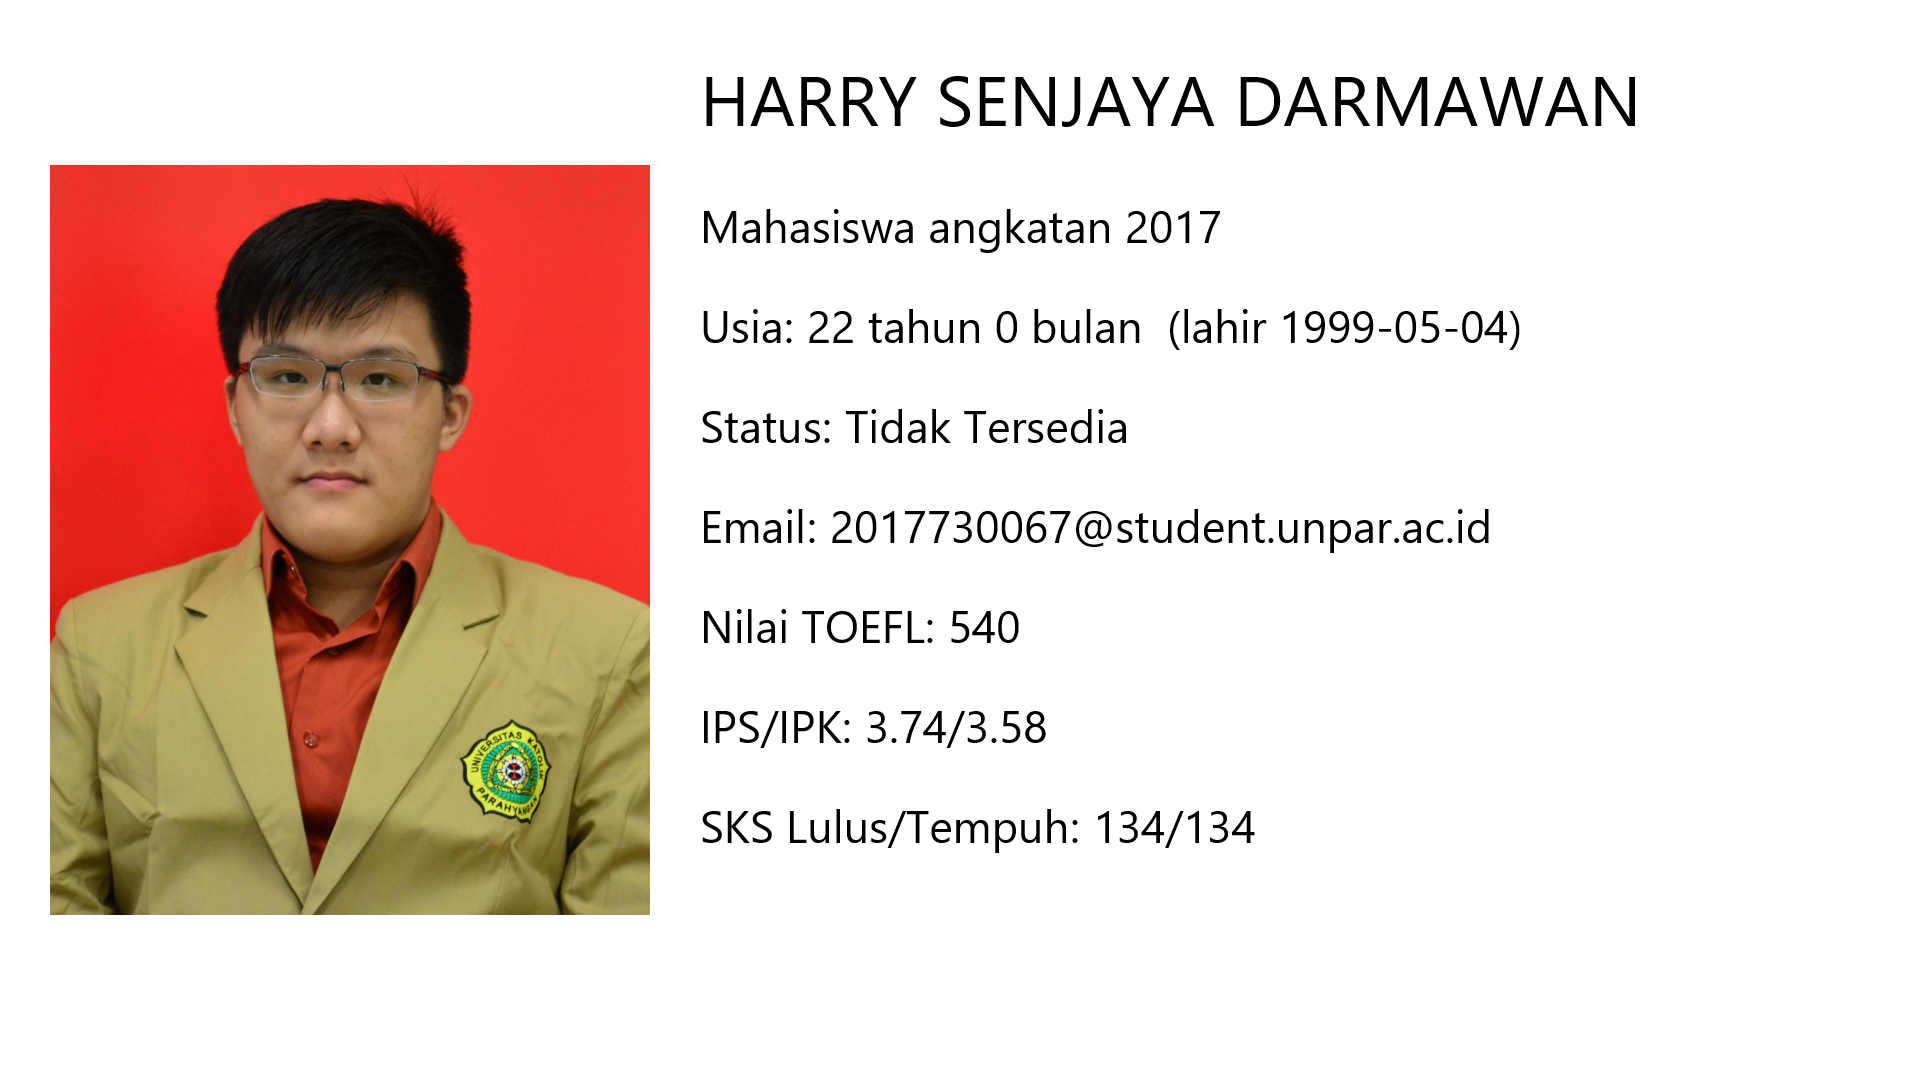
\includegraphics[scale=0.3]{Gambar/hasil.png}
	\caption{Tampilan \textit{Screensaver} Mahasiswa Pertama}
	\label{fig:5_hasil}
\end{figure}

\begin{figure}[H]
	\centering
	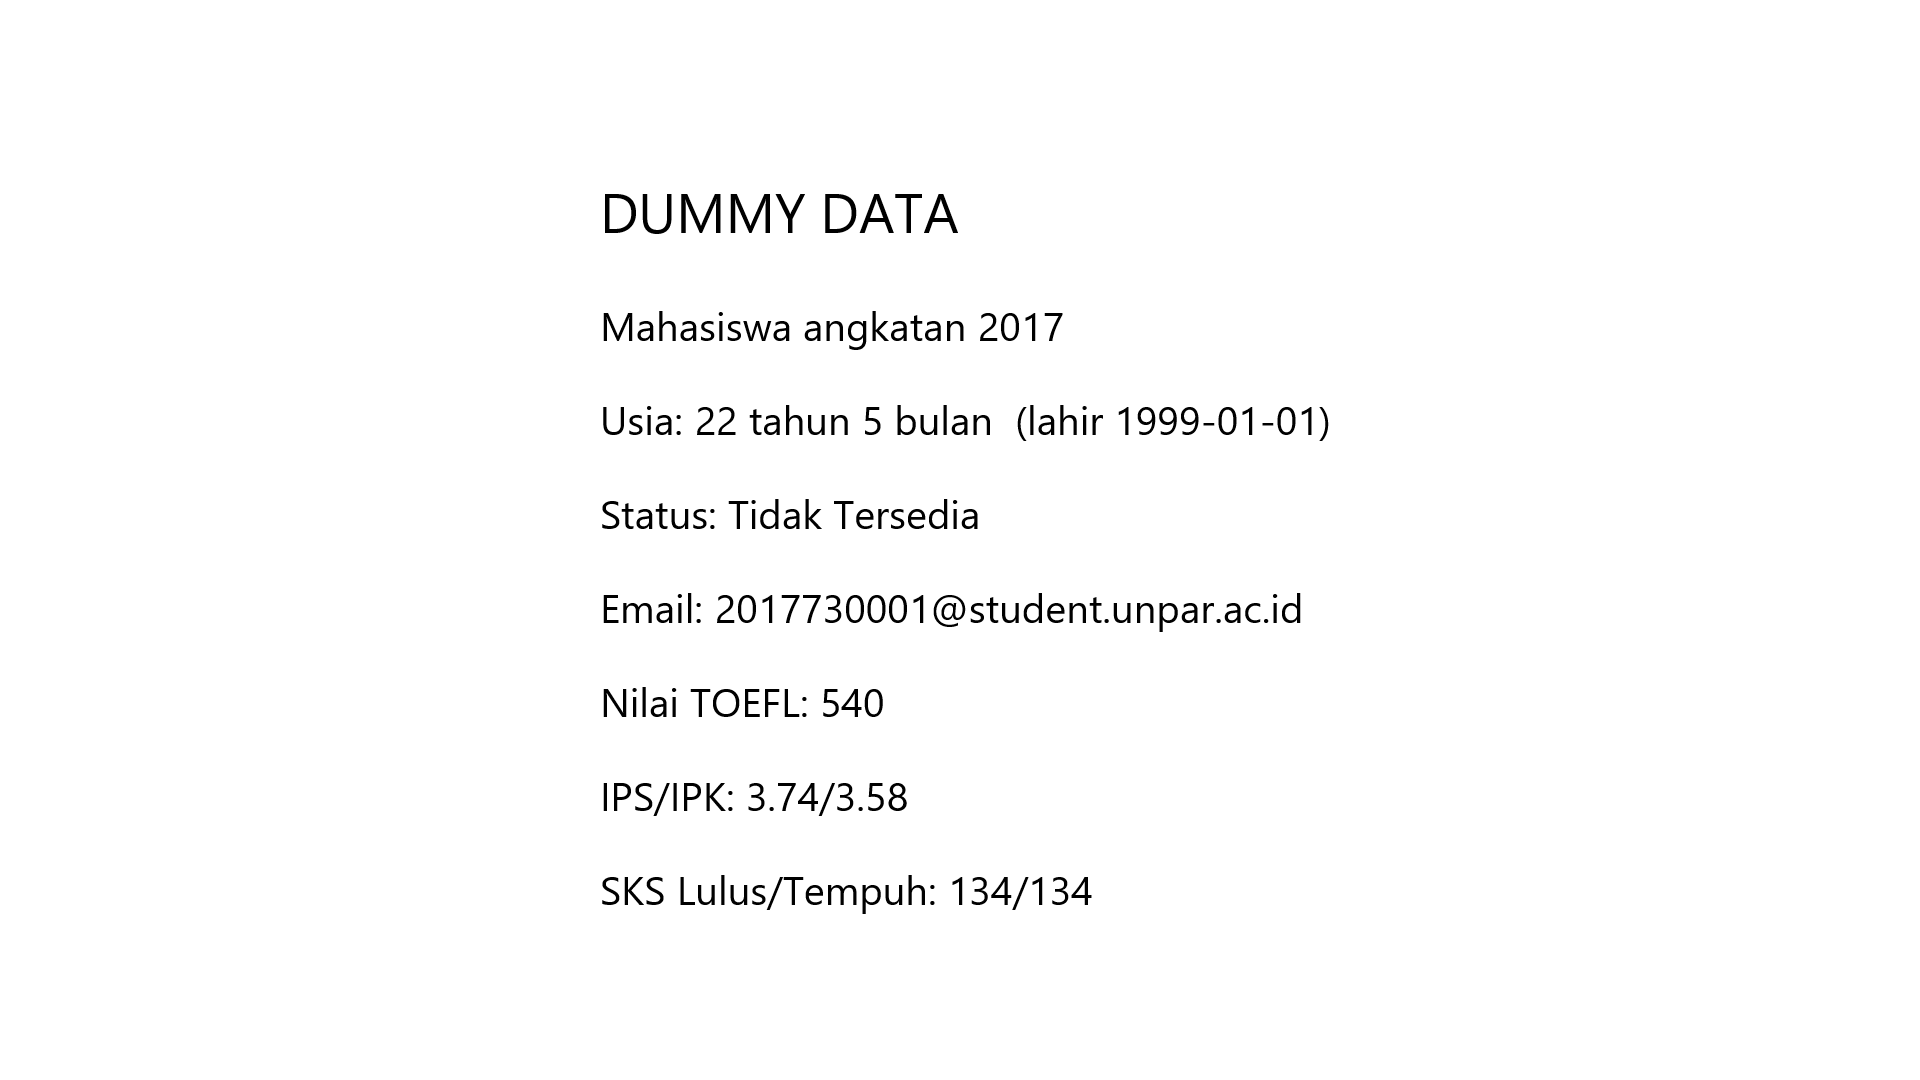
\includegraphics[scale=0.3]{Gambar/hasil2.png}
	\caption{Tampilan \textit{Screensaver} Mahasiswa Kedua}
	\label{fig:5_hasil2}
\end{figure}


\section{Pengujian}

\section{Pengujian Fungsional}
Pengujian fungsional dilakukan untuk mengetahui kesesuaian reaksi perangkat lunak dengan reaksi yang diharapkan berdasarkan aksi pengguna terhadap perangkat lunak. Tabel \ref{table:hasilFungsional} merupakan hasil pengujian perangkat lunak yang dilakukan di komputer penulis dengan spesifikasi berikut:
\begin{enumerate}
    \item \textit{Processor}: Intel Core i5-10300H
    \item \textit{Random Access Memory(RAM)}: 16 GB DDR4
    \item Sistem Operasi: Windows 10
    \item Resolusi Layar: 1920 x 1080
    \item Versi Java: 1.8.0\_291
\end{enumerate}

\begin{table}[H]
	\centering
	\caption{Tabel Pengujian Fungsional}
	\begin{tabular}{|p{0.5cm}| p{5.5cm}| p{5.5cm}| p{3cm}|} \hline
	No.	&	Aksi Pengguna	&	Reaksi yang diharapkan	&	Reaksi Perangkat Lunak \\ \hline
	1.	&	Dosen atau mahasiswa tidak menggunakan komputer selama beberapa saat. 	&	\textit{Screensaver} berjalan dengan menampilkan biodata dan data akademik mahasiswa secara umum.	&	sesuai	\\ \hline
	\end{tabular}
	\label{table:hasilFungsional}
\end{table}


\section{Pengujian Eksperimental}

\textit{Subbab ini ditulis oleh dosen pembimbing.}

Pengujian eksperimental dilakukan oleh dosen pembimbing, karena mahasiswa tidak memiliki akses ke SIAKAD apalagi ke data mahasiswa di luar penulis sendiri. Pengujian eksperimental dilakukan dengan melakukan \textit{git branching} dari hasil (hampir) final dari penulis di commit \texttt{d60be65}. Pengujian eksperimental dilakukan pada komputer dosen dengan spesifikasi seperti berikut\footnote{Idealnya pengujian dilakukan di komputer UNPAR dengan sistem operasi Microsoft Windows sehingga bisa benar-benar digunakan sebagai \textit{screensaver}. Namun, karena keadaan pandemi sehingga dosen tidak bisa mengunjungi UNPAR dan hanya bisa melakukan pengujian di rumah dengan komputer macOS}:

\begin{enumerate}
	\item Komputer: iMac (21.5-inch, Late 2013)
    \item Sistem Operasi: macOS Catalina 10.15.7
    \item \textit{Processor}: 2,7 GHz Quad-Core Intel Core i5
    \item \textit{Memory}: 8 GB 1600 MHz DDR3
    \item \textit{Graphics}: Intel Iris Pro 1536 MB
    \item Resolusi Layar: 1920 x 1080
    \item Versi Java: 1.8.0\_282
\end{enumerate}

Ada beberapa penyesuaian yang dilakukan oleh dosen pembimbing supaya \textit{screensaver} bisa dijalankan dengan cukup baik pada lingkungan dosen. Karena keterbatasan waktu, penyesuaian ini dilakukan tanpa berkoordinasi secara intensif dengan mahasiswa. Penyesuaian-penyesuaian tersebut antara lain:

\begin{enumerate}
	\item \textbf{Data diambil dari SIAKAD bukan dari Portal Akademik Mahasiswa.} Daftar mahasiswa yang diambil diacak urutannya sehingga saat ditampilkan tidak selalu dimulai dari angkatan tertua.
    \item \textbf{Upgrade versi SIAModels dari 4.0.0 menjadi 5.0.1.} Pada versi terbaru SIAModels, ada beberapa perbaikan, di mana salah satunya adalah \textit{bug} saat menentukan angkatan mahasiswa berdasarkan NPM nya. Perbaikan lainnya adalah pada perhitungan IPK dan IPS. SIAModels merupakan pustaka eksternal dan bukan merupakan bagian inti dari \textit{screensaver} yang dibuat.
    \item \textbf{Load data di \textit{thread} terpisah.} Pada program yang dibuat oleh mahasiswa, program hanya mengunduh satu data dari Portal Akademik Mahasiswa, yaitu data yang bersangkutan sendiri. Pada SIAKAD, diunduh banyak data dan ternyata menimbulkan masalah saat mengunduh data mahasiswa untuk ditampilkan pada slide berikutnya. Masalah muncul karena saat load data mahasiswa berikutnya, program menjadi tidak responsif. Oleh karena itu, saat menampilkan sebuah slide, program diubah supaya mengunduh data mahasiswa untuk slide berikutnya di latar belakang. Saat slide berikutnya ditampilkan, sudah tidak perlu melakukan pengunduhan kembali karena datanya sudah siap.
    \item \textbf{Saat mengulang ke mahasiswa pertama, tidak dilakukan load data kembali.}
    \item \textbf{Jika data mahasiswa belum siap ditampilkan, tidak maju ke slide berikutnya.}
    \item \textbf{\textit{Bugfix} untuk pembacaan bulan Februari.} Pada SIAKAD, ternyata bulan kedua dituliskan sebagai ``Pebruari'' dengan huruf ``P'', karena itu perlu penyesuaian sehingga mahasiswa dengan bulan lahir Februari dapat dibaca dengan baik.
\end{enumerate}

Perubahan lengkap kode dibandingkan dengan kode milik mahasiswa dapat dilihat di \textbf{TODO Harry tolong kode di bawah ini dipindah ke lampiran dan direfer dari sini}.

\begin{lstlisting}[language=diff, caption=Perbedaan kode dosen dengan mahasiswa, label=diff_dosen_mahasiswa]
diff --git a/ScreenSaver/src/main/java/id/ac/unpar/screensaver/PrimaryController.java b/ScreenSaver/src/main/java/id/ac/unpar/screensaver/PrimaryController.java
index 8ca4319..d8f3f26 100644
--- a/ScreenSaver/src/main/java/id/ac/unpar/screensaver/PrimaryController.java
+++ b/ScreenSaver/src/main/java/id/ac/unpar/screensaver/PrimaryController.java
@@ -1,7 +1,6 @@
 package id.ac.unpar.screensaver;
 
-//import id.ac.unpar.screensaver.siakad.SIAkadDataPuller;
-import id.ac.unpar.screensaver.studentportal.StudentPortalDataPuller;
+import id.ac.unpar.screensaver.siakad.SIAkadDataPuller;
 import id.ac.unpar.siamodels.Mahasiswa;
 import id.ac.unpar.siamodels.TahunSemester;
 import java.io.ByteArrayInputStream;
@@ -32,16 +31,22 @@ public class PrimaryController implements Initializable {
 
     private int indexOfMahasiswa = 0;
     private Mahasiswa[] listMahasiswa;
+    private boolean[] mahasiswaLoaded;
     private DataPuller puller;
 
     public int getIndexOfMahasiswa() {
         return indexOfMahasiswa;
     }
 
-    public void setIndexOfMahasiswa(int indexOfMahasiswa) {
+    public void setIndexOfMahasiswaAndPreload(int indexOfMahasiswa) {
         this.indexOfMahasiswa = indexOfMahasiswa;
+        if (!mahasiswaLoaded[indexOfMahasiswa]) {
+            new MahasiswaDetailPuller(listMahasiswa[indexOfMahasiswa]).start();
+        } else {
+            System.out.println("No longer pulling mahasiswa detail for " + listMahasiswa[indexOfMahasiswa].getNama() + " because already pulled before");
+        }
     }
-
+    
     public PrimaryController() throws IOException {
 
     }
@@ -49,71 +54,36 @@ public class PrimaryController implements Initializable {
     @Override
     public void initialize(URL url, ResourceBundle rb) {
         try {
-            puller = new StudentPortalDataPuller();
+            puller = new SIAkadDataPuller();
             listMahasiswa = puller.pullMahasiswas();
-        } catch (IllegalStateException ex) {
-            Logger.getLogger(PrimaryController.class.getName()).log(Level.SEVERE, null, ex);
-        }
-        if (listMahasiswa != null) {
-            try {
-                listMahasiswa[this.getIndexOfMahasiswa()] = puller.pullMahasiswaDetail(listMahasiswa[this.getIndexOfMahasiswa()]);
-                this.updateView(listMahasiswa[this.getIndexOfMahasiswa()]);
-                this.setIndexOfMahasiswa(this.getIndexOfMahasiswa() + 1);
-            } catch (IOException ex) {
-                Logger.getLogger(PrimaryController.class.getName()).log(Level.SEVERE, null, ex);
-            }
-        } else {
-            updateView();
-        }
-        Timeline timeline = new Timeline(
-                new KeyFrame(
-                        Duration.seconds(5),
-                        event -> {
-                            if (listMahasiswa == null) {
-                                updateView();
+            listMahasiswa[this.getIndexOfMahasiswa()] = puller.pullMahasiswaDetail(listMahasiswa[this.getIndexOfMahasiswa()]);
+            mahasiswaLoaded = new boolean[listMahasiswa.length];
+            this.updateView(listMahasiswa[this.getIndexOfMahasiswa()]);
+            this.setIndexOfMahasiswaAndPreload(this.getIndexOfMahasiswa() + 1);
+            Timeline timeline = new Timeline(
+                    new KeyFrame(
+                            Duration.seconds(15), // May need to adjust longer if internet is slow
+                            event -> {
                                 try {
-                                    puller = new StudentPortalDataPuller();
-                                    listMahasiswa = puller.pullMahasiswas();
-                                } catch (IllegalStateException ex) {
-                                    Logger.getLogger(PrimaryController.class.getName()).log(Level.SEVERE, null, ex);
-                                }
-                            } else {
-                                if (this.getIndexOfMahasiswa() == listMahasiswa.length) {
-                                    this.setIndexOfMahasiswa(0);
-                                } else {
-                                    if (listMahasiswa[this.getIndexOfMahasiswa()].getTanggalLahir() == null) {
-                                        listMahasiswa[this.getIndexOfMahasiswa()] = puller.pullMahasiswaDetail(listMahasiswa[this.getIndexOfMahasiswa()]);
-                                    }
-                                }
-                                if (listMahasiswa[this.getIndexOfMahasiswa()].getTanggalLahir() == null) {
-                                    updateView();
-                                } else {
-                                    try {
+                                    if (mahasiswaLoaded[this.getIndexOfMahasiswa()]) {
+                                        // Update view only if mahasiswa is loaded. Otherwise, wait for next turn
                                         this.updateView(listMahasiswa[this.getIndexOfMahasiswa()]);
-                                        this.setIndexOfMahasiswa(this.getIndexOfMahasiswa() + 1);
-                                    } catch (IOException ex) {
-                                        Logger.getLogger(PrimaryController.class.getName()).log(Level.SEVERE, null, ex);
+                                        this.setIndexOfMahasiswaAndPreload((this.getIndexOfMahasiswa() + 1) % listMahasiswa.length);
+                                    } else {
+                                        System.out.println("Mahasiswa " + listMahasiswa[this.getIndexOfMahasiswa()].getNama() + " is not ready. Waiting for next turn...");
                                     }
+                                } catch (IOException ex) {
+                                    Logger.getLogger(PrimaryController.class.getName()).log(Level.SEVERE, null, ex);
                                 }
                             }
-                        }
-                )
-        );
-        timeline.setCycleCount(Animation.INDEFINITE);
-        timeline.play();
+                    )
+            );
+            timeline.setCycleCount(Animation.INDEFINITE);
+            timeline.play();
 
-    }
-
-    public void updateView() {
-        this.foto.setVisible(false);
-        this.nama.setText("Pastikan koneksi internet berfungsi dengan normal!");
-        this.angkatan.setText("-");
-        this.usia.setText("-");
-        this.status.setText("-");
-        this.email.setText("-");
-        this.toefl.setText("-");
-        this.ipk.setText("-");
-        this.sks.setText("-");
+        } catch (IllegalStateException | IOException ex) {
+            Logger.getLogger(PrimaryController.class.getName()).log(Level.SEVERE, null, ex);
+        }
     }
 
     public void updateView(Mahasiswa mahasiswa) throws IOException {
@@ -129,13 +99,12 @@ public class PrimaryController implements Initializable {
         }
         this.nama.setText(mahasiswa.getNama());
         this.angkatan.setText(mahasiswa.getTahunAngkatan() + "");
-        this.usia.setText(Period.between(mahasiswa.getTanggalLahir(), LocalDate.now()).getYears() + " tahun " + Period.between(mahasiswa.getTanggalLahir(), LocalDate.now()).getMonths() + " bulan " + " (lahir " + mahasiswa.getTanggalLahir().toString() + ")");
-        if (mahasiswa.getStatus()!=null) {
-            this.status.setText(mahasiswa.getStatus().toString());
-        }
-        else{
-            this.status.setText("Tidak Tersedia");
-        }
+        this.usia.setText(
+            mahasiswa.getTanggalLahir() != null ?
+            (Period.between(mahasiswa.getTanggalLahir(), LocalDate.now()).getYears() + " tahun " + Period.between(mahasiswa.getTanggalLahir(), LocalDate.now()).getMonths() + " bulan (lahir " + mahasiswa.getTanggalLahir().toString() + ")") :
+            "Tidak tersedia"
+        );
+        this.status.setText(mahasiswa.getStatus() != null ? mahasiswa.getStatus().toString() : "Tidak Tersedia");
         this.email.setText(mahasiswa.getEmailAddress());
         if (mahasiswa.getNilaiTOEFL() != null && mahasiswa.getNilaiTOEFL().size() > 0) {
             this.toefl.setText(mahasiswa.getNilaiTOEFL().get(mahasiswa.getNilaiTOEFL().firstKey()).toString());
@@ -143,12 +112,34 @@ public class PrimaryController implements Initializable {
             this.toefl.setText("Tidak Tersedia");
         }
         TahunSemester tahunSemesterTerakhir = null;
-        for (Mahasiswa.Nilai nilai : mahasiswa.getRiwayatNilai()) {
+        for (Mahasiswa.Nilai nilai: mahasiswa.getRiwayatNilai()) {
             if (tahunSemesterTerakhir == null || nilai.getTahunSemester().compareTo(tahunSemesterTerakhir) > 0) {
                 tahunSemesterTerakhir = nilai.getTahunSemester();
             }
         }
-        this.ipk.setText(Math.round(mahasiswa.calculateIPS(tahunSemesterTerakhir) * 100.0) / 100.0 + "/" + Math.round(mahasiswa.calculateIPK() * 100.0) / 100.0);
+        this.ipk.setText(mahasiswa.getRiwayatNilai().isEmpty() ?
+                "Tidak tersedia" :
+                Math.round(mahasiswa.calculateIPS(tahunSemesterTerakhir) * 100.0) / 100.0 + "/" + Math.round(mahasiswa.calculateIPK() * 100.0) / 100.0
+        );
         this.sks.setText(+mahasiswa.calculateSKSLulus() + "/" + mahasiswa.calculateSKSTempuh(false));
     }
+
+    private class MahasiswaDetailPuller extends Thread {
+        private Mahasiswa mahasiswa;
+        public MahasiswaDetailPuller(Mahasiswa mahasiswa) {
+            this.mahasiswa = mahasiswa;
+        }
+        public void run() {
+            System.out.println("Pulling mahasiswa detail for " + mahasiswa.getNama());
+            puller.pullMahasiswaDetail(mahasiswa);
+            for (int i = 0; i < listMahasiswa.length; i++) {
+                if (listMahasiswa[i] == this.mahasiswa) {
+                    mahasiswaLoaded[i] = true;
+                    System.out.println("Pulled mahasiswa detail for " + mahasiswa.getNama() + " (index " + i + ")");
+                    break;
+                }
+            }
+            
+        }
+    }
 }
diff --git a/ScreenSaver/src/main/java/id/ac/unpar/screensaver/siakad/SIAkad.java b/ScreenSaver/src/main/java/id/ac/unpar/screensaver/siakad/SIAkad.java
index a1fcb3e..66a4512 100644
--- a/ScreenSaver/src/main/java/id/ac/unpar/screensaver/siakad/SIAkad.java
+++ b/ScreenSaver/src/main/java/id/ac/unpar/screensaver/siakad/SIAkad.java
@@ -53,7 +53,7 @@ public class SIAkad {
 	// it will be more flexible in case SIAkad uses different names compared
 	// to Java/OS's standard.
 	public static final String[] MONTH_NAMES = {
-		"Januari", "Februari", "Maret", "April", "Mei", "Juni", "Juli", "Agustus", "September", "Oktober", "November", "Desember"
+		"Januari", "Pebruari", "Maret", "April", "Mei", "Juni", "Juli", "Agustus", "September", "Oktober", "November", "Desember"
 	};
 
     Token token = null;
@@ -247,7 +247,7 @@ public class SIAkad {
 						StringTokenizer tokenizer = new StringTokenizer(fieldValue);
 						int day = Integer.parseInt(tokenizer.nextToken());
 						int month = Arrays.asList(MONTH_NAMES).indexOf(tokenizer.nextToken()) + 1;
-						if (month < 0) {
+						if (month <= 0) {
 							throw new ProtocolException("Month name not recognized in this date: " + fieldValue);
 						}
 						int year = Integer.parseInt(tokenizer.nextToken());
diff --git a/ScreenSaver/src/main/java/id/ac/unpar/screensaver/siakad/SIAkadDataPuller.java b/ScreenSaver/src/main/java/id/ac/unpar/screensaver/siakad/SIAkadDataPuller.java
index 82c35bc..27c0eed 100644
--- a/ScreenSaver/src/main/java/id/ac/unpar/screensaver/siakad/SIAkadDataPuller.java
+++ b/ScreenSaver/src/main/java/id/ac/unpar/screensaver/siakad/SIAkadDataPuller.java
@@ -10,10 +10,12 @@ import id.ac.unpar.siamodels.Mahasiswa;
 import java.io.FileNotFoundException;
 import java.io.FileReader;
 import java.io.IOException;
+import java.util.Collections;
 import java.util.List;
 import java.util.Properties;
 import java.util.logging.Level;
 import java.util.logging.Logger;
+import java.util.Random;
 
 /**
  *
@@ -36,8 +38,10 @@ public class SIAkadDataPuller extends DataPuller {
     @Override
     public Mahasiswa[] pullMahasiswas() {
         List<Mahasiswa> mahasiswas = null;
+        Random random = new Random(13); // "stable" random
         try {
             mahasiswas = siakad.requestMahasiswaList();
+            Collections.shuffle(mahasiswas, random);
         } catch (IllegalStateException ex) {
             Logger.getLogger(SIAkadDataPuller.class.getName()).log(Level.SEVERE, null, ex);
         } catch (IOException ex) {
diff --git a/ScreenSaver/src/main/java/id/ac/unpar/screensaver/studentportal/MultipleRequest.java b/ScreenSaver/src/main/java/id/ac/unpar/screensaver/studentportal/MultipleRequest.java
index 30b3207..d16618b 100644
--- a/ScreenSaver/src/main/java/id/ac/unpar/screensaver/studentportal/MultipleRequest.java
+++ b/ScreenSaver/src/main/java/id/ac/unpar/screensaver/studentportal/MultipleRequest.java
@@ -4,7 +4,7 @@ import id.ac.unpar.siamodels.Mahasiswa;
 import id.ac.unpar.siamodels.MataKuliah;
 import id.ac.unpar.siamodels.MataKuliahFactory;
 import id.ac.unpar.siamodels.TahunSemester;
-import jdk.nashorn.api.scripting.ScriptObjectMirror;
+// import jdk.nashorn.api.scripting.ScriptObjectMirror;
 import org.jsoup.Connection;
 import org.jsoup.Jsoup;
 import org.jsoup.nodes.Document;
@@ -50,17 +50,17 @@ public class MultipleRequest implements Runnable {
             Connection.Response resp = connection.execute();
             Document doc = resp.parse();
 
-            Element script = doc.select("script").get(doc.select("script").size() - 1);
+            Element script = doc.select("script").get(doc.select("script").size()-1);
             String scriptDataMataKuliah = script.html().substring(script.html().indexOf("var data_mata_kuliah = [];"), script.html().indexOf("var data_angket = [];"));
             engine.eval(scriptDataMataKuliah);
-            ScriptObjectMirror dataMataKuliah = (ScriptObjectMirror) engine.get("data_mata_kuliah");
+            // ScriptObjectMirror dataMataKuliah = (ScriptObjectMirror) engine.get("data_mata_kuliah");
             TahunSemester tahunSemesterNilai = new TahunSemester(Integer.parseInt(thn), sem.charAt(0));
-            for (Map.Entry<String, Object> mataKuliahEntry : dataMataKuliah.entrySet()) {
-                ScriptObjectMirror mataKuliah = (ScriptObjectMirror) mataKuliahEntry.getValue();
-                MataKuliah curr_mk = MataKuliahFactory.getInstance().createMataKuliah((String) mataKuliah.get("kode_mata_kuliah"), Integer.parseInt((String) mataKuliah.get("jumlah_sks")), (String) mataKuliah.get("nama_mata_kuliah"));
-                mahasiswa.getRiwayatNilai()
-                        .add(new Mahasiswa.Nilai(tahunSemesterNilai, curr_mk, (String) mataKuliah.get("na")));
-            }
+            // for (Map.Entry<String, Object> mataKuliahEntry : dataMataKuliah.entrySet()) {
+            //     ScriptObjectMirror mataKuliah = (ScriptObjectMirror) mataKuliahEntry.getValue();
+            //     MataKuliah curr_mk = MataKuliahFactory.getInstance().createMataKuliah((String) mataKuliah.get("kode_mata_kuliah"), Integer.parseInt((String) mataKuliah.get("jumlah_sks")), (String) mataKuliah.get("nama_mata_kuliah"));
+            //     mahasiswa.getRiwayatNilai()
+            //             .add(new Mahasiswa.Nilai(tahunSemesterNilai, curr_mk, (String) mataKuliah.get("na")));
+            // }
         } catch (IOException e) {
             e.printStackTrace();
         } catch (ScriptException se) {
diff --git a/ScreenSaver/src/main/java/id/ac/unpar/screensaver/studentportal/Scraper.java b/ScreenSaver/src/main/java/id/ac/unpar/screensaver/studentportal/Scraper.java
index 2786909..1f7a8ed 100644
--- a/ScreenSaver/src/main/java/id/ac/unpar/screensaver/studentportal/Scraper.java
+++ b/ScreenSaver/src/main/java/id/ac/unpar/screensaver/studentportal/Scraper.java
@@ -237,8 +237,9 @@ public class Scraper {
 
         Mahasiswa dummy = new Mahasiswa("2017730001");
         dummy.setNama("DUMMY DATA");
+        dummy.setJenisKelamin(JenisKelamin.PEREMPUAN);
+        dummy.setTanggalLahir(LocalDate.of(1, 1, 1));
         this.requestMahasiswaDetail(phpsessid, dummy);
-        dummy.setTanggalLahir(LocalDate.of(1999, Month.JANUARY, 1));
         mahasiswaList.add(dummy);
         Mahasiswa[] mahasiswaArray = new Mahasiswa[mahasiswaList.size()];
         for (int i = 0; i < mahasiswaArray.length; i++) {
diff --git a/ScreenSaver/src/main/java/id/ac/unpar/screensaver/studentportal/StudentPortalDataPuller.java b/ScreenSaver/src/main/java/id/ac/unpar/screensaver/studentportal/StudentPortalDataPuller.java
index e0e9e02..a165218 100644
--- a/ScreenSaver/src/main/java/id/ac/unpar/screensaver/studentportal/StudentPortalDataPuller.java
+++ b/ScreenSaver/src/main/java/id/ac/unpar/screensaver/studentportal/StudentPortalDataPuller.java
@@ -36,6 +36,7 @@ public class StudentPortalDataPuller extends DataPuller {
             this.mahasiswa = new Mahasiswa(npm);
             this.scraper = new Scraper();
             this.session = this.scraper.login(npm, password);
+
         } catch (IOException ex) {
             Logger.getLogger(PrimaryController.class.getName()).log(Level.SEVERE, null, ex);
         }
\end{lstlisting}

Setelah perbaikan-perbaikan di atas dilakukan, program dapat dijalankan dengan baik, dan untuk menampilkan 30 mahasiswa ``wali'' dari dosen pembimbing, dibutuhkan waktu sekitar 8 menit, di mana setelahnya mengulang kembali dari mahasiswa pertama. Beberapa hasil tangkapan layar dapat dilihat pada gambar \textbf{TODO Harry tolong sisipkan gambar-gambar dari video 5 mahasiswa yang sudah saya kirimkan sebelumnya}. Dosen sudah meminta izin kepada kelima mahasiswa tersebut untuk datanya dapat ditampilkan pada laporan ini, melalui e-mail.